\documentclass[a4paper, 12pt]{article}

\usepackage[utf8]{inputenc}
\usepackage{latexsym,amsfonts,amssymb,amsthm,amsmath}
\usepackage{setspace}
\usepackage{physics}
\usepackage{graphicx}
\usepackage{newtxtext}
\usepackage{extsizes}
\setlength{\parindent}{0in}
\setlength{\oddsidemargin}{0in}
\setlength{\textwidth}{6.5in}
\setlength{\textheight}{8.8in}
\setlength{\topmargin}{0in}
\setlength{\headheight}{8pt}

\onehalfspacing


\title{
  \vspace{-1.5cm}
  \textbf{Estimators}
  \vspace{-1.5cm}
}
\date{}

\begin{document}

\maketitle

\section{From Probability to Statistics}

In probability theory, mathematical models for stochastic phenomena are studied. The starting point is a known probabilistic model, and based on that model, probabilities for different events and outcomes are calculated.\\

Typical question: If a given model applies to the observed experiment, what is the
probability that a certain event will occur?\\

\textbf{Example 1.} A coin is tossed, assuming it is fair, i.e., the probability of landing heads is $p = 0.5$. The coin is tossed $5$ times.\\

\textbf{Question:} What is the probability of getting exactly 3 heads in 5 tosses?

In this case, the model is known - the number of heads is a random variable with
Binomial distribution $B(5, 0.5)$.\\


In statistics, the starting point is observed data for a given feature, representing a
random representative sample from the population. The model and its parameters are
considered unknown and need to be assumed, estimated, and/or verified. The goal is to
draw conclusions about the feature in the entire population based on the sample. The
direction of inference is reversed: from real data to a probabilistic model and its
parameters.

\textbf{Example 2.} A clinical trial is conducted with 100 patients given a new drug. For each patient, it is recorded whether the drug worked, resulting in a sample of 100 observations.\\

\textbf{Question:} What is the probability p that the drug works in the entire population? In this case, it is appropriate to assume that the data comes from a feature with a Bernoulli distribution $B(1, p)$. \textbf{The parameter $p$ is unknown and needs to be estimated based on the observed sample}.


\subsection{Probabilistic Model and Parameter}

Let the observed feature be modeled by a random variable $X$ with a distribution function $F(x)$ depending on an unknown parameter $\theta$. The parameter $\theta$ can be a scalar or a vector. We will denote the set of all possible values that the unknown parameter $\theta$ can take by $\Theta$. The set $\Theta$ is called the \textbf{parameter space}.\\

Example: $X \sim P(\lambda),\quad \theta=\lambda \quad \Theta=(0,\infty)$

$X\sim N(\mu, \sigma^2), \quad \theta=(\mu, \sigma^2), \quad \Theta=R \times R^+$

To emphasize the dependence on $\theta$, we will write $F(x,\theta)$ or $F(x,\theta)=P_\theta\{ X < x \}$. In fact, we do not have one, but a family of distributions $\{F(x, \theta) | \theta \in \Theta \}$


\subsection{Data Space and Parameter Space}

Let $X=(X_1, X_2, \dots , X_n)$ be a random sample from the feature $X$. The data space $W$ is the set of all possible realizations of the sample.\\

Example:

\begin{itemize}
  \item if $X\sim P(\lambda)$, then $W = \{ (x_1,x_2, \dots, x_n) | x_i \in \mathbb{N}, i=1,\dots,n \}$
  \item if $X\sim B(m,p)$, then $W = \{ (x_1,x_2, \dots, x_n) | 0 \leq x_i \leq m \in \mathbb{N}, i=1,\dots,n \}$
  \item if $X\sim N(\mu, \sigma^2)$, then $W = \mathbb{R}^n$
\end{itemize}

\textbf{Question:} How to estimate the unknown parameter $\theta$ based on the sample?
In this lecture, we will consider cases where the form of the distribution $F(x, \theta)$ is known, but the parameter $\theta$ (or some of its components) is unknown.

\subsection{Definition of an estimator}

\textbf{Definition: } Let $X = (X_1, X_2, \dots, X_n)$ be a random sample from the feature $X$, having distribution $F(x, \theta)$, and $\theta \in \Theta$ is an unknown parameter. An \textbf{estimator} (or point estimator) for the parameter $\theta$ is any statistic

\[\hat{\theta} = f(X_1, X_2, \dots, X_n) \]

where $f: W \rightarrow \Theta$ is a function depending only on the random sample and containing no unknown parameters. The estimator $\hat{\theta}$ is a random variable, and the specific value $\theta = f(x_1, \dots, x_n)$, obtained for a given realization of the sample $(x_1, \dots, x_n)$ is called an estimate of the parameter $\theta$.

\subsection{Methods for Obtaining Point Estimators}

The previous definition of an estimator is very broad. However, not every estimator is a good estimator - it needs to satisfy some properties, which we will mention later. Next, we will introduce simple methods for finding estimators, which often have desirable properties. We will talk about:

\begin{itemize}
  \item Methods of moments (MME)
  \item Methods of maximum likelihood (MLE)
\end{itemize}

\section{The Method of Moments Estimation}

How do we connect data with parameters?

Basic idea: It is known that sample characteristics are a good approximation for
population characteristics. The $k-th$ sample moment is an approximation for the
theoretical $k-th$ moment $\frac{1}{k}\sum_{}^{}X_i^k \approx E[X^k]$. Additionally theoretical moments depend on the unknown parameter $\theta$.\\

\textbf{The Methods of Moments}: If the model depends on $k$ unknown parameters, we take the first $k$ theoretical moments $m_k(\theta)=E_\theta (X^k)$ and equate them with the corresponding sample moments

\[ m_k(\theta) = \frac{1}{n}\sum_{i=1}^{n}X_i^k, \quad k=1,\dots, m \]

In this way we obtain a system of equations from which the estimator $\hat{\theta}$ is determined.

\section{Likelihood function}

Let $X = (X_1, X_2, \dots, X_n)$ be a random sample from feature $X$ with distribution $F(x, \theta)$, where $\theta \in \Theta$ is an unknown parameter (or vector of parameters). Let $p(x, \theta)$ denote the probability mass function (discrete case) or the probability density function (continuous case) of $X$ for a given $\theta$. For a fixed sample

\[ x = (x_1, x_2, \dots , x_n) \]

The \textbf{likelihood function} of parameter $\theta$ is defined as

\[ L(\theta; x) = \prod_{i=1}^{n}p(x_i, \theta) \]

The function $L(\theta; x)$ is considered a function of $\theta$, where the observed values $x_1, \dots , x_n$ are treated as constants.

\subsection{Interpretation of the Likelihood Function (Single observation)}

Let us have one observed value $x_1$ from $X \sim N(\mu, \sigma^2)$ for an unknown parameter $\mu$. The graph shows two possible densities for this model, for different values of parameter $\mu$. It is clear that the data $x_1$ is more likely (suitable) to come from the second distribution than from the first.\\

In fact, the likelihood function $L(\mu; x_1) = p(x_1|\mu, \sigma^2)$, will have a greater value in the second case.

\begin{figure}[h]
  \centering
  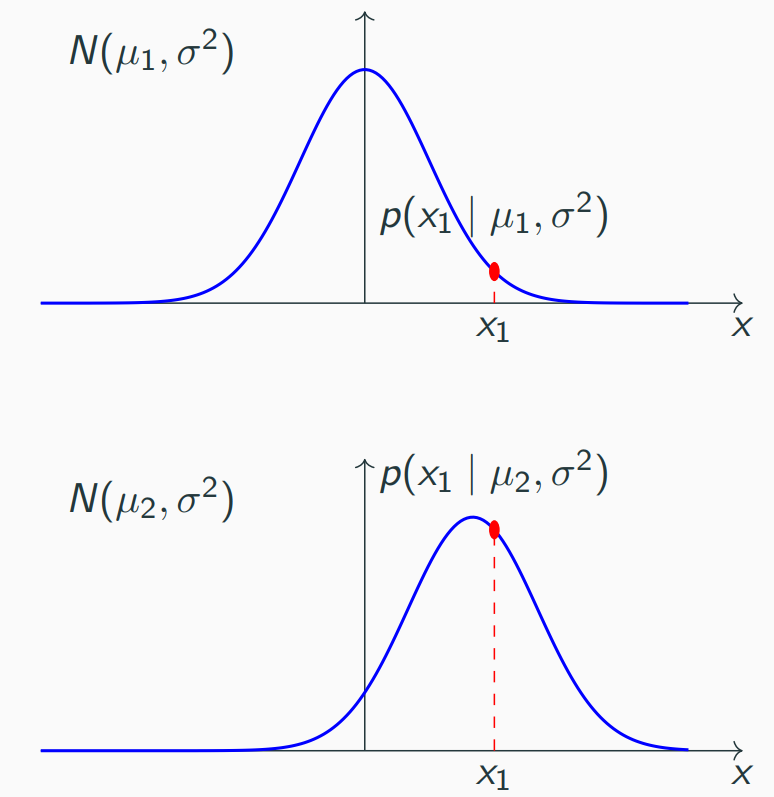
\includegraphics[width=0.4\textwidth]{image.png}
  \caption{}
  \label{fig:ll1}
\end{figure}


\subsection{Interpretation of the Likelihood Function (multiple observations)}

Let us have several observed values $x_1, x_2,x_3$ from the model $X \sim N(\mu, \sigma^2)$. For a fixed sample $(x_1, x_2, x_3) = \prod_{i=1}^{3}p(x_i | \mu, \sigma^2)$, where $(p(x, \mu,\sigma^2))$ is the density of the normal distribution.

Also for this sample, the likelihood function is greater in the second case, because the second distribution is more suitable for the given sample. But is it the most suitable distribution for this sample?\\

\textbf{Idea:} Find the distribution for which the likelihood function has the maximum value for the given sample.

\begin{figure}[h]
  \centering
  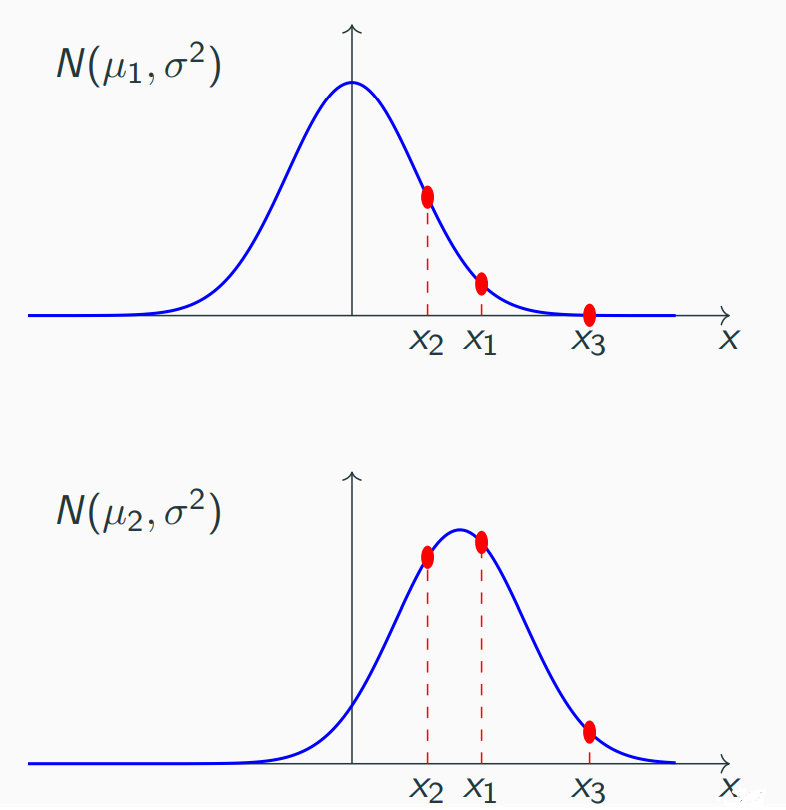
\includegraphics[width=0.4\textwidth]{image_2.png}
  \caption{}
  \label{fig:ll2}
\end{figure}

\section{Method of Maximum Likelihood (MLE)}

More precisely: The likelihood function is a function of the unknown parameter $\theta$. We want to find the value of the parameter for which this function assumes a maximum value, applying methods for finding the maximum of a function (if it exists). It is often easier to apply these methods to the logarithm of the likelihood function. We will consider the following procedure for finding the maximum:

\begin{itemize}
  \item Determine the function $L(\theta; x)$
  \item Take the logarithm: $l(\theta;x)=\ln L(\theta)$
  \item Find the derivative with respecet to $\theta$ and equate to 0 (find maximum):
  \[ \frac{dl(\theta;x)}{d\theta} = 0 \]
  \item Solve the equation for $\theta$.
\end{itemize}

\section{Properties of Estimators}

The estimator is a random variable, for a different sample we will get a different realization, i.e., estimate for the parameter. The question arises of how good this estimate is. \\

It is desirable for estimators to have the following properties:\\

\begin{itemize}
  \item \textbf{Ubiasedness}: $E[\hat{\theta}] = \theta$ -  the estimator hits the true value of the parameter on average. Example of unbiased estimators are $\overline{X}$ for $\mu=EX$ the expectation of $X$, and $S^2=\frac{1}{n-1}\sum_{i=1}^{n}(X_i-\overline{X})^2$ for $\sigma^2$, the variance of $X$.
  \item \textbf{Efficeincy}: If there are multiple estimators for the same parameters, the best one is the one with the smallest possible variance.

  \item \textbf{Consistency}: As the sample size grows ($n \rightarrow \infty$) we want the estimate to converge probabilistically to the true value.
\end{itemize}


\subsection{Precission and accuracy}

\begin{figure}[h]
  \centering
  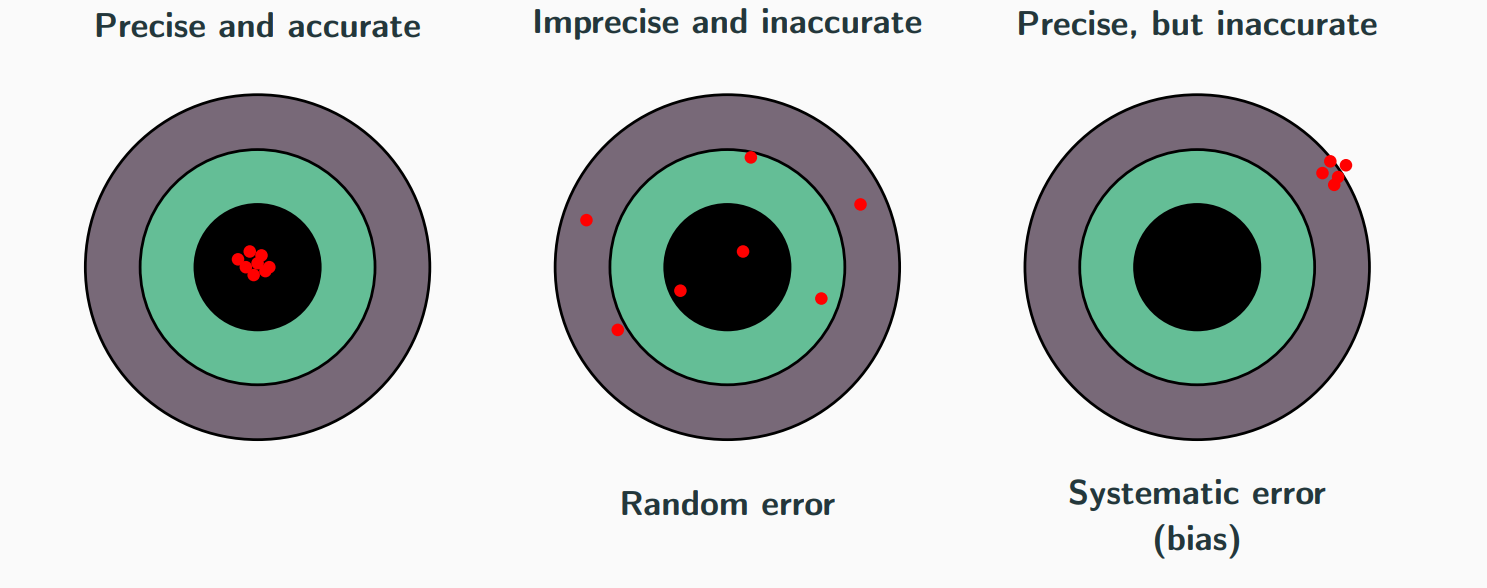
\includegraphics[width=0.7\textwidth]{image_3.png}
  \caption{}
  \label{fig:example_image}
\end{figure}


\section{Next steps...}

Estimation gives us the best guess for the parameters based on the sample, but we
cannot say how confident we are in these estimates. \textbf{Next step: Hypothesis testing} - a method to check if our estimates are statistically
significant or just a result of chance

\end{document}